% Options for packages loaded elsewhere
\PassOptionsToPackage{unicode,linktoc=all}{hyperref}
\PassOptionsToPackage{hyphens}{url}
\PassOptionsToPackage{dvipsnames,svgnames*,x11names*}{xcolor}
%
\documentclass[
  british,
  a4paper,
  rgb,
  dvipsnames,
  svgnames,
  hyphens]{article}
\usepackage{amsmath,amssymb}
\usepackage{lmodern}
\usepackage{iftex}
\ifPDFTeX
  \usepackage[T1]{fontenc}
  \usepackage[utf8]{inputenc}
  \usepackage{textcomp} % provide euro and other symbols
\else % if luatex or xetex
  \usepackage{unicode-math}
  \defaultfontfeatures{Scale=MatchLowercase}
  \defaultfontfeatures[\rmfamily]{Ligatures=TeX,Scale=1}
\fi
% Use upquote if available, for straight quotes in verbatim environments
\IfFileExists{upquote.sty}{\usepackage{upquote}}{}
\IfFileExists{microtype.sty}{% use microtype if available
  \usepackage[]{microtype}
  \UseMicrotypeSet[protrusion]{basicmath} % disable protrusion for tt fonts
}{}
\makeatletter
\@ifundefined{KOMAClassName}{% if non-KOMA class
  \IfFileExists{parskip.sty}{%
    \usepackage{parskip}
  }{% else
    \setlength{\parindent}{0pt}
    \setlength{\parskip}{6pt plus 2pt minus 1pt}}
}{% if KOMA class
  \KOMAoptions{parskip=half}}
\makeatother
\usepackage{xcolor}
\IfFileExists{xurl.sty}{\usepackage{xurl}}{} % add URL line breaks if available
\IfFileExists{bookmark.sty}{\usepackage{bookmark}}{\usepackage{hyperref}}
\hypersetup{
  pdftitle={Using Font Awesome in HTML and PDF documents},
  pdfauthor={R (Chandra) Chandrasekhar},
  pdflang={en-GB},
  colorlinks=true,
  linkcolor={DarkOliveGreen},
  filecolor={Purple},
  citecolor={DarkKhaki},
  urlcolor={Maroon},
  pdfcreator={LaTeX via pandoc}}
\urlstyle{same} % disable monospaced font for URLs
\usepackage[margin=25mm]{geometry}
\usepackage{color}
\usepackage{fancyvrb}
\newcommand{\VerbBar}{|}
\newcommand{\VERB}{\Verb[commandchars=\\\{\}]}
\DefineVerbatimEnvironment{Highlighting}{Verbatim}{commandchars=\\\{\}}
% Add ',fontsize=\small' for more characters per line
\usepackage{framed}
\definecolor{shadecolor}{RGB}{48,48,48}
\newenvironment{Shaded}{\begin{snugshade}}{\end{snugshade}}
\newcommand{\AlertTok}[1]{\textcolor[rgb]{1.00,0.81,0.69}{#1}}
\newcommand{\AnnotationTok}[1]{\textcolor[rgb]{0.50,0.62,0.50}{\textbf{#1}}}
\newcommand{\AttributeTok}[1]{\textcolor[rgb]{0.80,0.80,0.80}{#1}}
\newcommand{\BaseNTok}[1]{\textcolor[rgb]{0.86,0.64,0.64}{#1}}
\newcommand{\BuiltInTok}[1]{\textcolor[rgb]{0.80,0.80,0.80}{#1}}
\newcommand{\CharTok}[1]{\textcolor[rgb]{0.86,0.64,0.64}{#1}}
\newcommand{\CommentTok}[1]{\textcolor[rgb]{0.50,0.62,0.50}{#1}}
\newcommand{\CommentVarTok}[1]{\textcolor[rgb]{0.50,0.62,0.50}{\textbf{#1}}}
\newcommand{\ConstantTok}[1]{\textcolor[rgb]{0.86,0.64,0.64}{\textbf{#1}}}
\newcommand{\ControlFlowTok}[1]{\textcolor[rgb]{0.94,0.87,0.69}{#1}}
\newcommand{\DataTypeTok}[1]{\textcolor[rgb]{0.87,0.87,0.75}{#1}}
\newcommand{\DecValTok}[1]{\textcolor[rgb]{0.86,0.86,0.80}{#1}}
\newcommand{\DocumentationTok}[1]{\textcolor[rgb]{0.50,0.62,0.50}{#1}}
\newcommand{\ErrorTok}[1]{\textcolor[rgb]{0.76,0.75,0.62}{#1}}
\newcommand{\ExtensionTok}[1]{\textcolor[rgb]{0.80,0.80,0.80}{#1}}
\newcommand{\FloatTok}[1]{\textcolor[rgb]{0.75,0.75,0.82}{#1}}
\newcommand{\FunctionTok}[1]{\textcolor[rgb]{0.94,0.94,0.56}{#1}}
\newcommand{\ImportTok}[1]{\textcolor[rgb]{0.80,0.80,0.80}{#1}}
\newcommand{\InformationTok}[1]{\textcolor[rgb]{0.50,0.62,0.50}{\textbf{#1}}}
\newcommand{\KeywordTok}[1]{\textcolor[rgb]{0.94,0.87,0.69}{#1}}
\newcommand{\NormalTok}[1]{\textcolor[rgb]{0.80,0.80,0.80}{#1}}
\newcommand{\OperatorTok}[1]{\textcolor[rgb]{0.94,0.94,0.82}{#1}}
\newcommand{\OtherTok}[1]{\textcolor[rgb]{0.94,0.94,0.56}{#1}}
\newcommand{\PreprocessorTok}[1]{\textcolor[rgb]{1.00,0.81,0.69}{\textbf{#1}}}
\newcommand{\RegionMarkerTok}[1]{\textcolor[rgb]{0.80,0.80,0.80}{#1}}
\newcommand{\SpecialCharTok}[1]{\textcolor[rgb]{0.86,0.64,0.64}{#1}}
\newcommand{\SpecialStringTok}[1]{\textcolor[rgb]{0.80,0.58,0.58}{#1}}
\newcommand{\StringTok}[1]{\textcolor[rgb]{0.80,0.58,0.58}{#1}}
\newcommand{\VariableTok}[1]{\textcolor[rgb]{0.80,0.80,0.80}{#1}}
\newcommand{\VerbatimStringTok}[1]{\textcolor[rgb]{0.80,0.58,0.58}{#1}}
\newcommand{\WarningTok}[1]{\textcolor[rgb]{0.50,0.62,0.50}{\textbf{#1}}}
\usepackage{longtable,booktabs,array}
\usepackage{calc} % for calculating minipage widths
% Correct order of tables after \paragraph or \subparagraph
\usepackage{etoolbox}
\makeatletter
\patchcmd\longtable{\par}{\if@noskipsec\mbox{}\fi\par}{}{}
\makeatother
% Allow footnotes in longtable head/foot
\IfFileExists{footnotehyper.sty}{\usepackage{footnotehyper}}{\usepackage{footnote}}
\makesavenoteenv{longtable}
\usepackage{graphicx}
\makeatletter
\def\maxwidth{\ifdim\Gin@nat@width>\linewidth\linewidth\else\Gin@nat@width\fi}
\def\maxheight{\ifdim\Gin@nat@height>\textheight\textheight\else\Gin@nat@height\fi}
\makeatother
% Scale images if necessary, so that they will not overflow the page
% margins by default, and it is still possible to overwrite the defaults
% using explicit options in \includegraphics[width, height, ...]{}
\setkeys{Gin}{width=\maxwidth,height=\maxheight,keepaspectratio}
% Set default figure placement to htbp
\makeatletter
\def\fps@figure{htbp}
\makeatother
\setlength{\emergencystretch}{3em} % prevent overfull lines
\providecommand{\tightlist}{%
  \setlength{\itemsep}{0pt}\setlength{\parskip}{0pt}}
\setcounter{secnumdepth}{-\maxdimen} % remove section numbering
% $HOME/.pandoc/defaults/latex-header-includes.tex
% Common header includes for both lualatex and xelatex engines.
%
% \PassOptionsToPackage{rgb,dvipsnames,svgnames}{xcolor} % Done as classoptions in latex.yaml
\AtBeginEnvironment{quote}{\small}
\AtBeginEnvironment{longtable}{\centering}
%
\usepackage{setspace} % Font-specific spacing set as \setstretch [linestreetch in YAML] in font-specific selection file
%
\usepackage{etoolbox}
\usepackage{graphicx}
\usepackage{subcaption}
\usepackage{svg}
  \svgsetup{inkscapeversion=1}
%
\urlstyle{tt}
\usepackage[defaultlines=4,all]{nowidow}
%
%\usepackage[margins=raggedright]{floatrow} % Commented out since it can be problematic 
% Left aligns tables: Pandoc Tips and Tricks
%
% Adjust punctuation for footnotes
%
\usepackage{fnpct} % footnote _before_ punctuation reversed and adjusted.
  \setfnpct{after-dot-space=-0.15em,after-comma-space=-0.150em,add-punct-marks=;[0.06em]![0.06em]?[0.06em]:[0.06em]}
%
% Flexible fontsizes
%
\usepackage{fontsize}
%
\usepackage{pdflscape}
%
\usepackage[capitalize,noabbrev]{cleveref}
%
% Font-related; font-selection is in iles $HOME/.pandoc/defaults/[fontname]-font.tex
% 
\usepackage[main=british]{babel}
%
\newfontfamily{\emojifont}{Symbola} % since used generally; KIV proper solution
%
\usepackage{newunicodechar}
%\newcommand*{\myrightarrow}{\textsf{→}} % U+2192 or 0x2192
%\newunicodechar{→}{\myrightarrow}
% Also OK:
% \newunicodechar{→}{\texttt{→}} % U+2192 or 0x2192
\newunicodechar{→}{\texttt{→}}
%
% Default font features for all fontpec invoked font sets
%
\defaultfontfeatures{Mapping=TeX,Scale=MatchLowercase,Ligatures=TeX,Renderer=HarfBuzz}
% $HOME/.pandoc/defaults/merriweather-font.tex
% Standard font selection a la fontspec
% 
\setromanfont{Merriweather}
\setsansfont[BoldFont={* Semibold}]{Source Sans Pro}
\setmonofont[Scale=0.95]{Fira Mono}
\setmathfont[bold-style=ISO]{STIX Two Math}
\defaultfontfeatures{Mapping=TeX,Scale=MatchLowercase,Ligatures=TeX,Renderer=HarfBuzz}
%
\setstretch{1.2}
%
\usepackage{titling}
\usepackage{fancyhdr}
    \pagestyle{fancy}
    \fancyhead{}
    \fancyfoot{}
    \renewcommand{\headrulewidth}{0.2pt}
    \renewcommand{\footrulewidth}{0.2pt}
    \fancyhead[LO,RE]{\scshape\thetitle}
    \fancyfoot[CO,CE]{\footnotesize Copyright © 2006\textendash\the\year, R (Chandra) Chandrasekhar}
    \fancyfoot[RE,RO]{\thepage}
\newfontfamily{\regulariconfont}{Font Awesome 6 Free Regular}[Color=Grey]
\newfontfamily{\solidiconfont}{Font Awesome 6 Free Solid}[Color=Grey]
\newfontfamily{\brandsiconfont}{Font Awesome 6 Brands}[Color=Grey]
%
% Direct input of Unicode code points
%
\newcommand{\faEnvelope}{\regulariconfont\ ^^^^f0e0\normalfont}
\newcommand{\faMobile}{\solidiconfont\ ^^^^f3cd\normalfont}
\newcommand{\faLinkedin}{\brandsiconfont\ ^^^^f0e1\normalfont}
\newcommand{\faGithub}{\brandsiconfont\ ^^^^f09b\normalfont}
\newcommand{\faAtom}{\solidiconfont\ ^^^^f5d2\normalfont}
\newcommand{\faPaperPlaneRegular}{\regulariconfont\ ^^^^f1d8\normalfont}
\newcommand{\faPaperPlaneSolid}{\solidiconfont\ ^^^^f1d8\normalfont}

%
% The block below is commented out because of Tofu glyphs in HTML
%
% \newcommand{\faEnvelope}{\regulariconfont\ \normalfont}
% \newcommand{\faMobile}{\solidiconfont\ \normalfont}
% \newcommand{\faLinkedin}{\brandsiconfont\ \normalfont}
% \newcommand{\faGithub}{\brandsiconfont\ \normalfont}
\ifXeTeX
  % Load polyglossia as late as possible: uses bidi with RTL langages (e.g. Hebrew, Arabic)
  \usepackage{polyglossia}
  \setmainlanguage[variant=british]{english}
\else
  \usepackage[main=british]{babel}
% get rid of language-specific shorthands (see #6817):
\let\LanguageShortHands\languageshorthands
\def\languageshorthands#1{}
\fi
\ifLuaTeX
  \usepackage{selnolig}  % disable illegal ligatures
\fi

\title{Using Font Awesome in HTML and PDF documents}
\author{R (Chandra) Chandrasekhar}
\date{2022-01-20}

\begin{document}
\maketitle

\setlength{\parindent}{0pt} % block paragraph
\thispagestyle{empty}


\hypertarget{make-me-a-ruxe9sumuxe9-bake-me-a-ruxe9sumuxe9}{%
\subsection{Make me a résumé, bake me a
résumé}\label{make-me-a-ruxe9sumuxe9-bake-me-a-ruxe9sumuxe9}}

My friend, the polymath Solus ``Sol'' Simkin, sauntered into my
relaxation-cubicle one morning muttering cryptically, ``Make me a
résumé, bake me a résumé''. Noticing that I was not
\href{https://www.macmillandictionary.com/dictionary/british/be-on-the-same-page}{on
the same page}, he quickly asked, ``Do you know the difference between a
\href{https://www.thefreedictionary.com/curriculum+vitae}{CV (curriculum
vitae)} and a
\href{https://www.collinsdictionary.com/dictionary/english/résumé}{résumé}?''

When I said that it was the same thing, named differently across the
Atlantic divide, he grinned and said ``Gotcha!'' and remained
tantalizingly silent. After discussing other matters, he left, and I was
not to see him again for the better part of three days.

Meanwhile, I tried to buttress my case by mining the Web for the
differences in nuance and usage between a CV and a résumé. I sought and
pounced upon the charming book
\href{https://www.amazon.in/Divided-Common-Language-Christopher-Davies/dp/0618911626/}{\emph{Divided
By A Common Language: A Guide to British and American English}} by
Christopher Davies. In it, I discovered that a CV in the UK is called a
résumé in the US, but that a CV is typically longer than a résumé.
\emph{So, a condensed CV was indeed called a résumé in the US}. In
search of more details, I happened upon
\href{https://icc.ucdavis.edu/materials/résumé/résumécv}{this clear
explanation of the distinction between the two}.

Armed with this authoritative knowledge, I was prepared for Sol the next
time we met. Somewhat piqued, I asked him why he
\href{https://www.collinsdictionary.com/dictionary/english/snigger}{sniggered}
at me the last time, when I had been correct---even if not complete---in
my answer.

He apologized and said, ``I enjoy seeing you
\href{https://www.thefreedictionary.com/stew}{stew} sometimes. That's
what friends are for: to stew each other on occasion. Since we are into
culinary metaphors, let me share with you more details of that latest
commission.

``A youngish tech-type wandered into my office recently and said, `Make
me a résumé, bake me a résumé. But make it the best. I want a résumé to
outzip all others.'\,''

``I took him to mean that he wanted a short but piquant résumé, that so
stood out from all the others, that it would bag him whatever job he
fancied.''

I then asked him what his non-negotiable requirements were. His reply
was prompt, as though he had rehearsed for this very question. He said,
`I want dinky \href{https://fontawesome.com/}{\emph{Font Awesome}} icons

\includegraphics[width=0.025\textwidth,height=\textheight]{images/font-awesome.svg}
for my contact details.'

``Anything else?''

``Only that the résumé must be generated from the \emph{same} source
document to give \emph{identical} outputs in three formats: PDF, HTML,
and \texttt{docx}. That will make maintenance a
\href{https://www.merriam-webster.com/dictionary/cinch}{cinch}. No other
stipulations.''

\hypertarget{the-yeast-gets-to-work}{%
\subsection{The yeast gets to work}\label{the-yeast-gets-to-work}}

Sol continued: ``For the world of me, I didn't know what Font Awesome
was, let alone its icons. I discovered that it was in its sixth
incarnation by the time I got acquainted with it. In any case, I didn't
think it would strain my brain to insert graphical icons into a résumé
to satisfy a client-stipulation.

But how wrong I was! It cost me a week in time just to investigate and
meet the single source document requirement, let alone the Font Awesome
icons. In the end, though,
\href{https://idioms.thefreedictionary.com/slog\%2Fslug+it+outslogging}{slogging
and slugging it out}, I managed the feat. I am sure you don't want to
hear about it.''

He knew my weakness---\emph{I crave the thing denied}---and used it to
tease me. So, I had to coax and cajole Sol to narrate to me yet another
of his \href{https://www.lexico.com/definition/scriptorial}{scriptorial}
escapades, leaving out no essential clue so, that I could track his
mental trajectory and experience for myself
\href{https://www.collinsdictionary.com/dictionary/english/the-thrill-of-the-chase}{the
thrill of the chase}. Exuding the essence of amicability, Sol agreed to
treat me to another of his tales of cerebral sleuthing.

\hypertarget{font-awesome-and-unicode-real-estate}{%
\subsection{Font Awesome and Unicode
real-estate}\label{font-awesome-and-unicode-real-estate}}

Sol recounted that Font Awesome was an
\href{https://www.merriam-webster.com/dictionary/atypical}{atypical}
font. Its \href{https://en.wikipedia.org/wiki/Glyph}{glyphs} did not fit
into standard \href{https://en.wikipedia.org/wiki/Unicode_block}{Unicode
blocks} reserved for the symbols of a natural language or academic
discipline. The fonts did not represent a finite alphabet, but were
rather an extensible set of hieroglyphs, not unlike
\href{https://en.wikipedia.org/wiki/Emoticon}{emoticons}. And while the
latter have been recognized and given their own
\href{https://en.wikipedia.org/wiki/Emoticons_(Unicode_block)}{Emoticon
Unicode block}, the Font Awesome icons are yet to receive their due
recognition through allocation of dedicated Unicode real estate.

Accordingly, Font Awesome started out using unallocated areas of
Unicode, defined as the
\href{https://www.unicode.org/faq/private_use.html}{Private Use Area
(PUA)}, which at present can accommodate a total of 137,468 private-use
characters. Given that Font Awesome is open-ended at present, it remains
to be seen whether this unallocated Unicode PUA will prove sufficient
for its future growth.

Moreover, the PUA may legitimately be used by other fonts as well. So,
the problem of collisions---two \emph{different} fonts using the
\emph{same} Unicode location in the PUA---remains a possible and
unresolved issue. Such ambiguity might give rise to unpredictable output
due to glyph clashes.

Moreover, Font Awesome has in the past strayed away from the PUA, and
\href{https://fontawesome.com/v5.15/how-to-use/on-the-web/advanced/css-pseudo-elements}{encroached
upon the domains reserved for other purposes}. This has thankfully been
corrected in more recent versions. Sol decided to avoid altogether the
complications of unwitting encroachment by using the
\href{https://fontawesome.com/download\#}{latest version} of Font
Awesome.

\hypertarget{glyphs-characters-numbers-or-images}{%
\subsection{Glyphs: characters, numbers, or
images?}\label{glyphs-characters-numbers-or-images}}

When Sol downloaded the desktop and web versions of the latest Font
Awesome free version, he noticed when rummaging into the downloaded
files that each glyph had a name, not unlike the name we give to letters
of the Latin alphabet. The downloaded fonts shared a
\href{https://www.collinsdictionary.com/dictionary/english/triune}{triune}
property:

\begin{enumerate}
\item
  Each glyph had a \emph{name}. For example,
  
\includegraphics[width=0.02\textwidth,height=\textheight]{images/font-awesome.svg}
  was called, not unsurprisingly, \emph{font-awesome} since the flag it
  embodies is the branding chosen by Font Awesome for itself.
\item
  As an \href{https://en.wikipedia.org/wiki/OpenType}{OpenType} (OTF) or
  \href{https://en.wikipedia.org/wiki/TrueType}{TrueType} (TTF) font,
  each glyph had a
  \href{https://en.wikipedia.org/wiki/Code_point}{\emph{Unicode code
  point}}. For example the \emph{font-awesome} icon had the
  \href{https://en.wikipedia.org/wiki/Hexadecimal}{hexadecimal} location
  code \texttt{f2b4} or \texttt{F2B4}.
\item
  In addition to its expression as a glyph in an OTF/TTF font, each
  symbol was also available as a \emph{scalable vector image} in
  \href{https://developer.mozilla.org/en-US/docs/Web/SVG}{SVG} format.
  This is unsurprising as we are dealing with a character set of icons
  or images.
\end{enumerate}

Sol told me that he was not at first aware of this triple
correspondence, but that he accidentally stumbled upon it as he delved
deeper into the downloaded Font Awesome files. He said that the triad of
a named glyph, a Unicode point, and an SVG icon each came to his rescue
for output to PDF, HTML, and \texttt{docx}.

Sol made a
\href{https://www.lexico.com/definition/mule-headed}{mule-headed}
decision after this discovery: he would not fall back upon the SVG
versions for his assignment, for it would defeat the very idea of a font
if he started using the SVG icons that could as well have been arbitrary
images. He wanted a \emph{true} challenge rather than a staged one.

\hypertarget{two-additional-layers-of-identity}{%
\subsubsection{Two additional layers of
identity}\label{two-additional-layers-of-identity}}

Font Awesome is distributed in two versions: a free version available at
no charge, and a paid version called \texttt{Font\ Awesome\ Pro}. Over
and above that, the free version comes in three \emph{flavours}:

\begin{itemize}
\tightlist
\item
  \texttt{Regular},
\item
  \texttt{Solid}, and
\item
  \texttt{Brands}.
\end{itemize}

The first two contained icons for general use while the third was
explicitly for the logos of brands. Sol confided that skill was needed
to invoke the correct flavour of free fonts from the appropriate font
file to get the desired output.
``\href{https://idioms.thefreedictionary.com/a+miss+is+as+good+as+a+mile}{A
miss is as good as a mile, mind you},'' he said.

With this convoluted introduction, Sol excused himself to rush away for
an appointment. It would be a week before he took up the dangling thread
of his narrative again.

\hypertarget{single-source-file-to-multiple-targets}{%
\subsection{Single source file to multiple
targets}\label{single-source-file-to-multiple-targets}}

When next we met, Sol started explaining how he fulfilled the
stipulation of a single source file that would generate three target
files in three different formats: PDF, HTML, and \texttt{docx}.

Sol had relaxed in his \emph{cogitation hammock} and decided that he
would ruminate on this vital requirement. His first thought was to do it
all in
\href{https://www.microsoft.com/en-in/microsoft-365/word}{Microsoft
Word} and use its built-in conversion capabilities to generate the PDF
and HTML outputs. But there was a mute dissension at the background of
his mind that refused to be silenced. He decided to let the creative
yeast do its work undisturbed, and left the problem to ferment.

A few days later, it struck him that if Microsoft Word changed its
default format as a result of program development in the same way that
PDF version 1.4 gave way to PDF 1.5, or as HTML 4 deferred to HTML 5,
his work would not survive the
\href{https://www.youtube.com/watch?v=FTLylKsI8xY\&feature=emb_imp_woyt}{march
of time}. The more he thought about it, the more he became convinced
that the most granitic of formats would be \emph{pure text encoded in}
\href{https://en.wikipedia.org/wiki/UTF-8}{\emph{UTF 8}}.

He rued that---by giving up on using Microsoft Word as his base
document---he was now further away from his goal than ever before. He
now had to convert text into three formats, not two, and that too,
unaided by any professional program. The responsibility for this was his
alone.

There was a nagging temptation to revert in silent acquiescence to
Microsoft Word and
\href{https://www.phrases.org.uk/meanings/put-paid-to.html}{put paid} to
the issue. But each time, he had to contend with the disquiet in his
heart. It was a heavy feeling that he was running away from a hard
problem rather than facing it
\href{https://www.dictionary.com/browse/manful}{manfully}. He felt that
he would sooner or later be forced to convert a single plain text source
to multiple formatted documents: a challenge better faced sooner rather
than later.

\hypertarget{pandoc-to-the-rescue}{%
\subsubsection{Pandoc to the rescue}\label{pandoc-to-the-rescue}}

In his quest for a plain text input format, Sol first thought of
\href{https://en.wikipedia.org/wiki/LaTeX}{LaTeX} with which he was
familiar. It had several paths to convert output to PDF and also HTML.
While there was no guarantee of foolproof conversion, it seemed
promising. But the
\href{https://dictionary.cambridge.org/dictionary/english/dealbreaker}{dealbreaker}
was that there was no route to Microsoft Word's \texttt{.docx} format.
Sadly, he let his firstborn inspiration take flight.

He next surfed the Web for
\href{https://themightyprogrammer.dev/article/parsing}{parsing} programs
that wielded the power of computer science to guarantee that the
conversion would be \emph{almost} error-free if indeed not
\emph{totally} error-free. He needed to convert formatted text into a
structure like an
\href{https://en.wikipedia.org/wiki/Abstract_syntax_tree}{abstract
syntax tree} that could again be re-converted into formatted text. He
thought it strange that the most robust or efficient route from \emph{A}
to \emph{B} was sometimes through \emph{C}, but granted that it could be
so sometimes.

He spent the next day sweeping the Web for ``format converters using
parsing''. But the results he got were about \emph{data} parsing:
extraction of possibly useful data from documents. He decided to set
that right by specifying ``document format converters using parsing''.
But again he got mired in results for \emph{parsing of data extracted
from documents}.

Somewhat vexed, he tried ``document format converters'' and was led to a
promising cloud-based service called
\href{https://convertio.co/document-converter/}{Convertio}. Another was
\href{https://document.online-convert.com/}{Online-Convert.com}. But the
more he thought about it, the less inclined was he to use such services.
For one, he could have stuck to his original idea of using Microsoft
Word as his input format, and using its built-in converters for PDF and
HTML. No uploading to the cloud. No security hassles. No fuss. No muss.
But that was a road he had already decided to avoid.

He stared at his non-negotiable specifications once again. It was then
that he realized that two of the three stipulated formats, PDF and HTML,
were publicly specified, standardized specifications. Only the
\texttt{.docx} format was proprietary. Sol decided to search using
``open source document format converter''. The first result showed
\href{https://pandoc.org/}{Pandoc}.

He first checked whether Pandoc could take in plain text and put out the
three desired formats. After confirming that it could, he realized that
it would be prudent to start off with
\href{https://daringfireball.net/projects/markdown/}{Markdown} and use
that almost-plain-text source to generate the other three. He decided to
use Pandoc's Markdown, which was a sophisticated outgrowth from the
original Markdown.

He next took a look at the somewhat
\href{https://pandoc.org/diagram.svg}{intricate network diagram} on the
right of the Pandoc home page. The plethora of formats available
convinced him that Pandoc would future-proof his work in case even more
output formats were required by his client later on. Sol decided to
pitch his format conversion tent squarely on the Pandoc field.

\hypertarget{a-skeleton-in-markdown}{%
\subsection{A skeleton in Markdown}\label{a-skeleton-in-markdown}}

``A résumé must have content: in this case, my client's'', said Sol,
stating the blindingly obvious. ``But for our intellectual excursion, we
shall skip the content and replace it by abstract placeholders. That
way, I keep my client's details confidential, and we will not
\href{https://idioms.thefreedictionary.com/muddy+the+waters}{muddy the
waters} with needless detail. In fact, I propose to show you only
\emph{one} simple line of pseudo content, which is also \emph{the single
line} where Font Awesome makes its debut.''

Sol then showed a snippet of a Pandoc Markdown text file with the pseudo
content shown below:

\begin{Shaded}
\begin{Highlighting}[]
\NormalTok{:::::center}
\CommentTok{[}\OtherTok{Joe Bloggs}\CommentTok{]}\NormalTok{\{.larger\}\textbackslash{}}
\NormalTok{[}\CommentTok{[}\OtherTok{mail icon}\CommentTok{]} \OtherTok{\textless{}joebloggs@mydomain.com\textgreater{}}\NormalTok{ |}
\CommentTok{[}\OtherTok{mobile icon}\CommentTok{]}\NormalTok{ +1{-}555{-}3456{-}7890 |}
\CommentTok{[}\OtherTok{LinkedIn icon}\CommentTok{] [LinkedIn]}\NormalTok{ |}
\CommentTok{[}\OtherTok{Github icon}\CommentTok{] [Github]}\NormalTok{]\{.smaller\}}
\NormalTok{:::::}
\end{Highlighting}
\end{Shaded}

He explained that the four icons above were a sufficient complement of
Awesome Font icons to demonstrate
\href{https://en.wikipedia.org/wiki/Proof_of_concept}{proof of concept},
and that any additions would simply translate to `more of the same'.
``Now that the scaffolding is in place, let us get to
\href{https://idioms.thefreedictionary.com/meat+of+the+matter}{the meat
of the matter}.''

\hypertarget{the-atom-icon}{%
\subsubsection{The atom icon}\label{the-atom-icon}}

Schooled as he was Greek philosophy, Sol decided that the atom would be
the fittest icon to begin his acquaintance with Font Awesome. He would
experiment and build his knowledge atom by atom.

He went to the \href{https://fontawesome.com/v6.0/icons}{latest icons
page}, selected \texttt{Free} on the left checkbox and typed ``atom''.
From the gallery of 32 icons, he selected the one that best met his
expectations. The popup screen he saw is shown below:

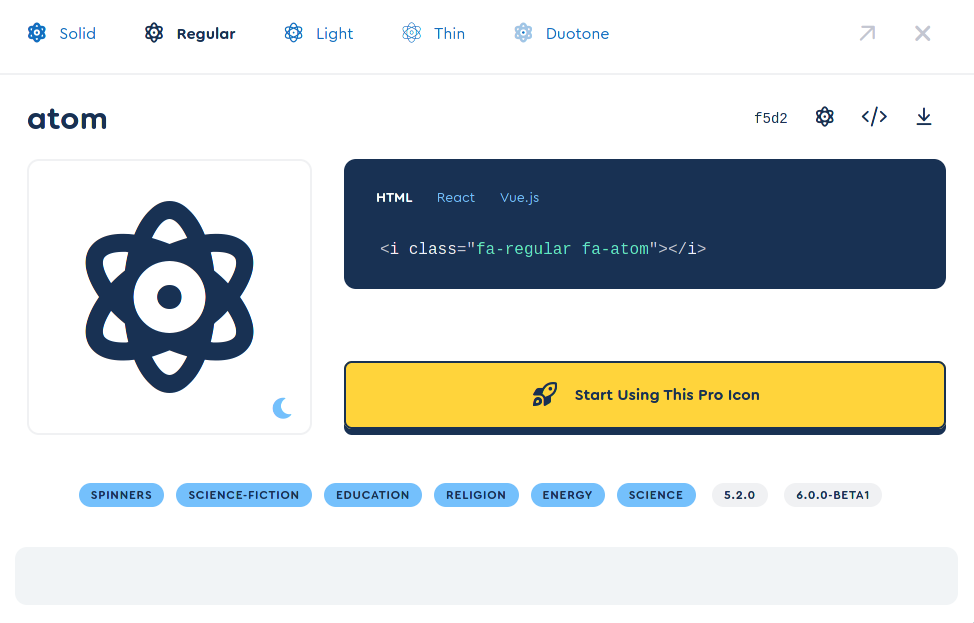
\includegraphics[width=0.9\textwidth,height=\textheight]{images/atom.png}

Its Unicode code point was \texttt{f5d2}, its name was \texttt{atom},
its SVG icon file was called \texttt{atom.svg}, and the glyph could be
copied by clicking on the picture of the atom next to the Unicode value.
He was seeing the \texttt{Solid} flavour of the icon; other variants
were not included in the free version he had downloaded. Interestingly,
the code snippet for HTML was also given with the icon as:

\begin{Shaded}
\begin{Highlighting}[]
\KeywordTok{\textless{}i} \ErrorTok{class}\OtherTok{=}\StringTok{"fa{-}solid fa{-}atom"}\KeywordTok{\textgreater{}\textless{}/i\textgreater{}}
\end{Highlighting}
\end{Shaded}

where the
\href{https://developer.mozilla.org/en-US/docs/Web/HTML/Element/i}{\texttt{\textless{}i\textgreater{}}
stood for ``Idiomatic Text element''}.

Not one to take things at face value, Sol immediately tested the HTML
invocation on his browser
\href{https://www.thefreedictionary.com/hoping+against+hope}{hoping
against hope} that the given incantation \emph{alone} could
automagically conjure up the atom icon. When it did not, Sol muttered to
himself that more work was in store.

He wracked his brain for the reason for failure. After some effort, he
decided to simulate his web browser in his head by attempting to `act'
like it. ``I will assume that the given incantation is meaningful and
correct. But it is only an HTML fragment. If I were a web browser, what
would I need \emph{in addition to the incantation} to display the atom
icon? How does my browser \emph{know} what that incantation means? It
was not born with that knowledge pre-programmed into it somehow.
\emph{So who tells it what the incantation means, and where to look for
that icon?}'' With that thought uppermost in his mind, Sol retired for
the night.

\hypertarget{a-second-look-at-the-atom-icon}{%
\subsubsection{A second look at the atom
icon}\label{a-second-look-at-the-atom-icon}}

When Sol took a second look at the problem the next day, he was aghast
that he had missed many clues strewn all over the Font Awesome website
that would have guided him in the right direction. Not one to waste time
on regret, he started to assemble the given sequence of instructions and
follow them meticulously.

Sol loaded \href{https://fontawesome.com/v6.0}{this page} to be greeted
by two large selection buttons:

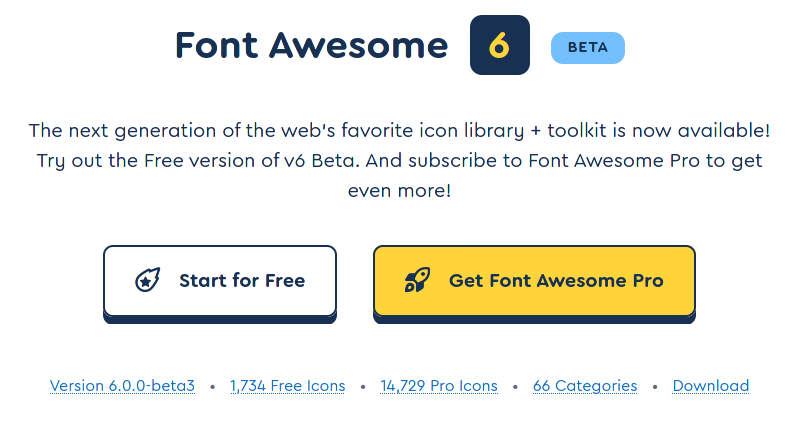
\includegraphics[width=0.9\textwidth,height=\textheight]{images/start-for-free.png}

And when he selected
\href{https://fontawesome.com/v6.0/docs/web/setup/quick-start}{\texttt{Start\ for\ Free}},
he was led to a clear and
\href{https://fontawesome.com/v6.0/docs/web/setup/quick-start}{detailed
algorithm} on how to set up and use Font Awesome. Central to everything
was a simple
\href{https://en.wikipedia.org/wiki/One-liner_program}{one-liner}
\emph{customized for him} that yielded an HTML script when he clicked
\href{https://fontawesome.com/kits}{\texttt{Set\ up\ a\ Kit}}. The
script he got looked like this:

\begin{Shaded}
\begin{Highlighting}[]
\KeywordTok{\textless{}script} \ErrorTok{src}\OtherTok{=}\StringTok{"https://kit.fontawesome.com/[some{-}hex{-}digits].js"}
\OtherTok{    crossorigin=}\StringTok{"anonymous"}\KeywordTok{\textgreater{}\textless{}/script\textgreater{}}
\end{Highlighting}
\end{Shaded}

The script was supposed to be included in the
\texttt{\textless{}head\textgreater{}} of the HTML document. This one
line was the automagical incantation that Sol was looking for the
previous night. He tried it out on the \texttt{atom} icon. The text

\begin{Shaded}
\begin{Highlighting}[]
\KeywordTok{\textless{}i} \ErrorTok{class}\OtherTok{=}\StringTok{"fa{-}solid fa{-}atom"}\KeywordTok{\textgreater{}\textless{}/i\textgreater{}}
\end{Highlighting}
\end{Shaded}

yielded the icon \faAtom Voila!

The maroon\footnote{The PDF version of this font on the PDF version of
  this blog will be shown in grey as explained later.} colour arose from
a little CSS fragment that set the colour of the icon to maroon with

\begin{Shaded}
\begin{Highlighting}[]
\FunctionTok{.fa{-}solid}\NormalTok{ \{}
    \KeywordTok{color}\NormalTok{: }\ConstantTok{maroon}\OperatorTok{;}
\NormalTok{\}}
\end{Highlighting}
\end{Shaded}

This meant that \emph{all} Font Awesome \texttt{Solid} icons will show
up in maroon. If he wanted another \texttt{Solid} icon, say,
\texttt{paper-plane}, to show up in a blue-green colour, he would need
to override this setting with

\begin{Shaded}
\begin{Highlighting}[]
\FunctionTok{.fa{-}paper{-}plane}\NormalTok{ \{}
    \KeywordTok{color}\NormalTok{: }\ConstantTok{\#004369}\OperatorTok{;} \CommentTok{/* a deep shade of blue{-}green */}
\NormalTok{\}}
\end{Highlighting}
\end{Shaded}

to get a correctly coloured \texttt{paper-plane} icon from the
\texttt{Solid} flavour: \faPaperPlaneSolid . Indeed, even the version
from the \texttt{Regular} flavour would be in the same colour:
\faPaperPlaneRegular

\hypertarget{the-four-icon-alphabet}{%
\subsubsection{The four-icon alphabet}\label{the-four-icon-alphabet}}

Inspired by his success and encouraged by the ease of use of the icons
in HTML, Sol decided on the four-icon alphabet he would use for the
placeholders in his single-line résumé template. He laid out his data
so:

\begin{longtable}[]{@{}lllcc@{}}
\toprule
Unicode & Flavour & Name & Icon & Glyph \\
\midrule
\endhead
\texttt{f0e0} & Regular & \texttt{envelope} & &
\regulariconfont \normalfont \\
\texttt{f3cd} & Solid & \texttt{mobile-screen-button} & &
\solidiconfont \normalfont \\
\texttt{f0e1} & Brands & \texttt{linkedin-in} & & \brandsiconfont 
\normalfont \\
\texttt{f09b} & Brands & \texttt{github} & & \brandsiconfont 
\normalfont \\
\bottomrule
\end{longtable}

The column headed \texttt{Icons} was generated by the
\texttt{\textless{}i\ class="fa-...\ fa-..."\textgreater{}\textless{}/i\textgreater{}}
code while that labelled \texttt{Glyphs} contained the relevant glyph
directly copied from the popup.

Note that the mobile phone icon available in the free version was only
from the \texttt{Solid} flavour, whereas the envelope icon was available
in both the \texttt{Regular} and \texttt{Solid} flavours.

The icon colour was set by this CSS fragment, and applies only to the
\texttt{Icons} column:

\begin{Shaded}
\begin{Highlighting}[]
\FunctionTok{.fa{-}envelope}\OperatorTok{,} \FunctionTok{.fa{-}mobile{-}screen{-}button}\OperatorTok{,} \FunctionTok{.fa{-}linkedin{-}in}\OperatorTok{,} \FunctionTok{.fa{-}github}\NormalTok{ \{}
  \KeywordTok{color}\NormalTok{: }\ConstantTok{\#2e8bc0}\OperatorTok{;}
\NormalTok{\}}
\end{Highlighting}
\end{Shaded}

``Notice that the Glyph column\footnote{In the PDF version of the blog,
  it is the \texttt{Icon} column that is blank, whereas the
  \texttt{Glyph} column, containing the glyph, shows up.} only shows
\href{https://en.wikipedia.org/wiki/Noto_fonts\#Origin_of_Noto_name}{tofu
rectangles}'' continued Sol. ``This is because the browser has not been
instructed on which fonts to use for these specialized Unicode
characters from the PUA.''

``On my text editor, the glyphs I see in column 5 correspond exactly
with those displayed on the web page in column 4. To get the browser to
display the glyphs directly, without the
\texttt{\textless{}i\ class=...\textgreater{}\textless{}/i\textgreater{}}
invocation, requires more effort than I am willing to expend right now.
So, I took the easy route here.'' \emojifont {😉} \normalfont

\hypertarget{wrapping-up-the-html-version}{%
\subsection{Wrapping up the HTML
version}\label{wrapping-up-the-html-version}}

``Wait a minute,'' I said. What about the PDF and the \texttt{.docx}
versions?

``Patience! Patience,'' he replied. ``Markdown was originally devised to
play well with HTML. Pandoc has carried that ball far and wide into many
other formats. All I have told you thus far applies only to HTML. Let me
wrap it up first before moving on to PDF. In HTML, the one-line résumé
template in Markdown looks like this:

\begin{Shaded}
\begin{Highlighting}[]
\NormalTok{Joe Bloggs}
\KeywordTok{\textless{}i} \ErrorTok{class}\OtherTok{=}\StringTok{"fa{-}regular fa{-}envelope"}\KeywordTok{\textgreater{}\textless{}/i\textgreater{}} \KeywordTok{\textless{}joebloggs}\ErrorTok{@mydomain.com}\KeywordTok{\textgreater{}}\NormalTok{\textbackslash{}}
\KeywordTok{\textless{}i} \ErrorTok{class}\OtherTok{=}\StringTok{"fa{-}solid fa{-}mobile{-}screen{-}button"}\KeywordTok{\textgreater{}\textless{}/i\textgreater{}}\NormalTok{ +1{-}555{-}3456{-}7890\textbackslash{}}
\KeywordTok{\textless{}i} \ErrorTok{class}\OtherTok{=}\StringTok{"fa{-}brands fa{-}linkedin{-}in"}\KeywordTok{\textgreater{}\textless{}/i\textgreater{}}\NormalTok{ [LinkedIn account of Joe Bloggs]()\textbackslash{}}
\KeywordTok{\textless{}i} \ErrorTok{class}\OtherTok{=}\StringTok{"fa{-}brands fa{-}github"}\KeywordTok{\textgreater{}\textless{}/i\textgreater{}}\NormalTok{ [Github account of Joe Bloggs]()}
\end{Highlighting}
\end{Shaded}

which \href{auxiliary/opening-html}{appears like this}\footnote{This
  file could not be named as \texttt{opening-html.html} because of an
  operational quirk in the \href{https://blog.getpelican.com/}{Pelican
  Static Site Generator} being used on this site. Accordingly, the
  \texttt{.html} file extension has been left out. Save this file,
  rename it as \texttt{opening-html.html}, open it in a Web browser, and
  verify for yourself the claim made here.}:

\begin{figure}
\centering

\includegraphics[width=0.9\textwidth,height=\textheight]{images/opening-html.png}
\caption{The Font Awesome icons take on the blue colour above.}
\end{figure}

The styling, like font size and text-alignment, is accomplished using
CSS.'' With a look of accomplishment, Sol ended his narration and asked
me whether I honestly wanted to hear how the PDF version was generated.
When I nodded in eager agreement, he said he would take up the thread on
another day.

\hypertarget{the-route-to-pdf}{%
\subsection{The route to PDF}\label{the-route-to-pdf}}

``The single most important difference between HTML on the one hand, and
PDF and \texttt{.docx} on the other is that the latter two are bound to
a physical paper size. The maximum width of text in these two formats
are constrained by the type of paper used. I will assume either
\href{https://en.wikipedia.org/wiki/ISO_216\#A_series}{A4} or
\href{https://en.wikipedia.org/wiki/Letter_(paper_size)}{US letter}
sizes for the output.

``The second aspect of these latter two formats is that the requisite
font must reside on the device generating the output. Moreover it is
possible, with some effort, to
\href{https://en.wikipedia.org/wiki/Font_embedding}{embed the fonts}
within the document so that another person viewing the document on
another device \emph{without} the fonts on his or her system can still
view the document with precisely the intended fonts.''

With this preamble, Sol started on his story of how he got the PDF
version of the one-line résumé template.

\hypertarget{does-the-font-exist-on-my-desktop}{%
\subsubsection{Does the font exist on my
desktop?}\label{does-the-font-exist-on-my-desktop}}

He said he used a combination of Pandoc and the
\href{https://www.tug.org/begin.html}{TeX/LaTeX} typesetting eco-system
to generate the PDF. A very important first step was to confirm that the
desired glyphs were indeed provided by the font in question. For that,
Sol used
\href{https://ctan.org/pkg/albatross?lang=en}{\texttt{albatross}}. This
utility may be invoked either with the Unicode glyph itself as argument,
or with the Unicode code point prefixed with either \texttt{0x} or
\texttt{U+}.

Sol tried \texttt{albatross\ U+f3cd} (for the
\texttt{mobile-screen-button}) and got
\texttt{Font\ Awesome\ 6\ Free\ Solid} as the only result. But when he
typed \texttt{albatross\ 0xf0e0} (for the \texttt{envelope}) he got a
total of seven fonts, including \texttt{Font\ Awesome\ 6\ Free\ Regular}
and also \texttt{Font\ Awesome\ 6\ Free\ Solid}. This was why one should
specify the font to be used---to avoid the same glyphs from a different
font, possibly with an incompatible style, or worse, of an entirely
different glyph as well, because the glyph is in the PUA area of the
font.

The results he got were sufficient for Sol to write the following
fragments in LaTeX:

\begin{Shaded}
\begin{Highlighting}[]
\FunctionTok{\textbackslash{}newfontfamily}\NormalTok{\{}\FunctionTok{\textbackslash{}regulariconfont}\NormalTok{\}\{Font Awesome 6 Free Regular\}[Color=Grey]}
\FunctionTok{\textbackslash{}newfontfamily}\NormalTok{\{}\FunctionTok{\textbackslash{}solidiconfont}\NormalTok{\}\{Font Awesome 6 Free Solid\}[Color=Grey]}
\FunctionTok{\textbackslash{}newfontfamily}\NormalTok{\{}\FunctionTok{\textbackslash{}brandsiconfont}\NormalTok{\}\{Font Awesome 6 Brands\}[Color=Grey]}
\CommentTok{\%}
\FunctionTok{\textbackslash{}newcommand}\NormalTok{\{}\ExtensionTok{\textbackslash{}faEnvelope}\NormalTok{\}\{}\FunctionTok{\textbackslash{}regulariconfont\textbackslash{} }\NormalTok{\^{}\^{}\^{}\^{}f0e0}\FunctionTok{\textbackslash{}normalfont}\NormalTok{\}}
\FunctionTok{\textbackslash{}newcommand}\NormalTok{\{}\ExtensionTok{\textbackslash{}faMobile}\NormalTok{\}\{}\FunctionTok{\textbackslash{}solidiconfont\textbackslash{} }\NormalTok{\^{}\^{}\^{}\^{}f3cd}\FunctionTok{\textbackslash{}normalfont}\NormalTok{\}}
\FunctionTok{\textbackslash{}newcommand}\NormalTok{\{}\ExtensionTok{\textbackslash{}faLinkedin}\NormalTok{\}\{}\FunctionTok{\textbackslash{}brandsiconfont\textbackslash{} }\NormalTok{\^{}\^{}\^{}\^{}f0e1}\FunctionTok{\textbackslash{}normalfont}\NormalTok{\}}
\FunctionTok{\textbackslash{}newcommand}\NormalTok{\{}\ExtensionTok{\textbackslash{}faGithub}\NormalTok{\}\{}\FunctionTok{\textbackslash{}brandsiconfont\textbackslash{} }\NormalTok{\^{}\^{}\^{}\^{}f09b}\FunctionTok{\textbackslash{}normalfont}\NormalTok{\}}
\NormalTok{...}
\KeywordTok{\textbackslash{}begin}\NormalTok{\{}\ExtensionTok{center}\NormalTok{\}}
\NormalTok{\{}\FunctionTok{\textbackslash{}Large}\NormalTok{ Joe Bloggs\}}\FunctionTok{\textbackslash{}\textbackslash{}}
\NormalTok{\{}\FunctionTok{\textbackslash{}small} \FunctionTok{\textbackslash{}faEnvelope\textbackslash{}}
\FunctionTok{\textbackslash{}href}\NormalTok{\{mailto: joebloggs@mydomain.com\}\{joebloggs@mydomain.com\} |}
\FunctionTok{\textbackslash{}faMobile\textbackslash{} }\NormalTok{+1{-}555{-}3456{-}7890 |}
\FunctionTok{\textbackslash{}faLinkedin\textbackslash{} \textbackslash{}href}\NormalTok{\{https://www.linkedin.com/\}\{LinkedIn\} |}
\FunctionTok{\textbackslash{}faGithub\textbackslash{} \textbackslash{}href}\NormalTok{\{https://github.com/\}\{GitHub\}\}}\FunctionTok{\textbackslash{}normalsize}
\KeywordTok{\textbackslash{}end}\NormalTok{\{}\ExtensionTok{center}\NormalTok{\}}
\end{Highlighting}
\end{Shaded}

The resulting PDF content, imaged below, matches the HTML output shown
earlier.

\begin{figure}
\centering

\includegraphics[width=0.9\textwidth,height=\textheight]{images/opening-pdf.png}
\caption{Note that the Font Awesome icons are grey, following the
settings above.}
\end{figure}

\hypertarget{file-manifest}{%
\subsection{File manifest}\label{file-manifest}}

Sol concluded by saying that the following files, in the order of their
invocation in the \href{auxiliary/make-html-pdf}{\texttt{make-html-pdf}}
script, were used to generate the HTML and PDF output from Pandoc's
Markdown source:

\begin{enumerate}
\tightlist
\item
  \href{auxiliary/html-defaults.yaml}{\texttt{html-defaults.yaml}}
\item
  \href{auxiliary/html-header-includes}{\texttt{html-header-includes}}
\item
  \href{auxiliary/awesome.css}{\texttt{awesome.css}}
\item
  \href{auxiliary/opening-html}{\texttt{opening-html}}
\item
  \href{auxiliary/opening-html.txt}{\texttt{opening-html.txt}}
\item
  \href{auxiliary/latex-defaults.yaml}{\texttt{latex-defaults.yaml}}
\item
  \href{auxiliary/latex-font.yaml}{\texttt{latex-font.yaml}}
\item
  \href{auxiliary/latex-header-includes.tex}{\texttt{latex-header-includes.tex}}
\item
  \href{auxiliary/latex-before-body-includes.tex}{\texttt{latex-before-body-includes.tex}}
\item
  \href{auxiliary/opening-latex.pdf}{\texttt{opening-latex.pdf}}
\item
  \href{auxiliary/opening-latex.txt}{\texttt{opening-latex.txt}}
\end{enumerate}

It bears noting that the input files for the two formats,
\texttt{opening-latex.txt} and \texttt{opening-html.txt}, are indeed
non-identical. In that sense the challenge has not been met. But given
that the first line of the résumé may be concatenated with the rest of
the résumé, \emph{which is unchanged for both formats}, the challenge
has been successfully, in spirit if not in letter.

I was lost in admiration for Sol's tenacity, which bent fonts and
typesetting systems to his will, to generate near-identical output in
two different, ubiquitous formats. Even if the effort expended on this
single line of text was disproportionate to the outcome, the experience
earned was worth every ounce of effort.

\hypertarget{the-.docx-output}{%
\subsection{\texorpdfstring{The \texttt{.docx}
output}{The .docx output}}\label{the-.docx-output}}

It was some weeks before I met Sol again in an unhurried setting. I then
reminded him to finish his saga with Font Awesome by explaining how he
generated the \texttt{.docx} version of the résumé opening. Sol squinted
his eyes and addressed me seriously: ``Do you \emph{really} want to know
that? If you do, grab a chair and have some water handy, in case you
feel dizzy. \emojifont {😉} \normalfont''

With that admonitory preamble, Sol launched into the third part of his
exploit: to get a \texttt{.docx} fragment visually identical to the HTML
and PDF versions from the same Markdown source. It was more a marathon
than a sprint, and required fortitude of body and mind.

``I do not claim to be an expert on Microsoft Word or its \texttt{.docx}
format. But I do have a secret weapon, or should I say, a secret agent:
my paternal cousin, once removed, Hieronymus Septimus Simkin, who is
affectionately known to me as Seven. He has been steeped and pickled in
the brine of Microsoft software since he barely started walking, and he
is my go-to resource on all matters relating to Windows applications.

``The road to \texttt{.docx} is a little convoluted and very tedious.
Why don't I try to get Seven to brief you himself. Let us agree to hold
that story in abeyance for another day and another blog.

\hypertarget{feedback}{%
\subsection{Feedback}\label{feedback}}

Please \href{mailto:feedback.swanlotus@gmail.com}{email me} your
comments and corrections.

\noindent A PDF version of this article is
\href{./using-font-awesome.pdf}{available for download here}.\footnote{Note
  that some icons that show up in the HTML version are missing from the
  PDF version of the blog, and vice versa. It was too tedious to make
  them feature-identical. One workaround would have been to use scaled
  SVG icons for both output formats, instead of HTML snippets for HTML,
  and OTF fonts invoked by Unicode code points, for LaTeX, but Sol felt
  that was a \href{https://www.thefreedictionary.com/cop+out}{cop out}.
  The opening of the résumé is almost identical in the HTML and PDF
  versions, and that was the challenge that was to be fulfilled: so no
  rules were broken in playing the game. \emojifont {😅} \normalfont}



\end{document}
